\documentclass[a4paper, 12pt]{article}
\usepackage{temp}
\usepackage{epsfig,graphicx,subfigure,amsthm,amsmath, float, xcolor, changepage, mathtools, textcomp, hyperref, bm, amssymb, tcolorbox, tikz, setspace, mathrsfs}
\usepackage[shortlabels]{enumitem}
\usepackage[bottom]{footmisc}
\usepackage{xepersian}
\settextfont[Scale=1]{XBZar}
%\setdigitfont{XBZar}
\setlatintextfont[Scale=0.9]{Times New Roman}
\hypersetup{
	colorlinks=true,
	urlcolor=blue!70!black
}

\newcommand{\myeq}[1]
{\stackrel{\mathclap{{\scriptsize \mbox{#1}}}}{=}}

%\normalfont

\doublespacing
\begin{document}
\handout
{یادگیری ماشین}
{نیم‌سال اول ۰۱\lr{-}۰۰}
{دکتر عباس حسینی}
{دانشکده مهندسی کامپیوتر}
{تمرین چهارم}
{محمد‌جواد هزاره}
{98101074}
\noindent
\\ [-6em]
\section*{سوال ۱}
\begin{enumerate}[A)]
	\item
	بردار $\bm{\hat{n}}$ را بردار یکه در راستای متناظر با $w$ای در نظر می‌گیریم که $B$ را بدست می‌آورد. به عبارتی خواهیم داشت:
	\[
	\forall i \in \{1, \cdots, m\}: y_i\langle B\bm{\hat{n}}, x_i\rangle \ge 1 \qquad (\ast)
	\]
	فرض کنیم الگوریتم $k$ بار اجرا می‌شود. هدف پیدا کردن کرانی برای $k$ است. حال اگر در مرحله‌ی $t$ام، داده‌ی $j$ام اشتباه دسته‌بندی شده باشد، آن‌گاه
	$\bm{w^{t+1}} = \bm{w^{t}} + y_j\bm{x_j}$.
	بنابراین داریم:
	\[
	\begin{aligned}
	\begin{aligned}
		\langle\bm{w^{t+1}}, B\bm{\hat{n}}\rangle &= B \langle\bm{w^t + y_j\bm{x_j}}, \bm{\hat{n}}\rangle \\
			&= B \left(\langle\bm{w^t}, \bm{\hat{n}}\rangle + \langle y_j\bm{x_j}, \bm{\hat{n}}\rangle\right)
	\end{aligned} \\[1.5em]
	\begin{aligned}
		\implies\langle\bm{w^{t+1}}, \bm{\hat{n}} \rangle &= \langle\bm{w^t}, \bm{\hat{n}}\rangle + \frac{1}{B} \langle y_j\bm{x_j}, B\bm{\hat{n}}\rangle \\
		&\ge \langle\bm{w^t}, \bm{\hat{n}}\rangle + \frac{1}{B}
	\end{aligned}
	\end{aligned}
	\]
	که خط آخر با توجه به $(\ast)$ نتیجه شده است. حال با توجه به استقرا و این‌که 
	$\bm{w^1} = \bm{0}$
	، برای هر $t$ در بازه‌ی ۱ تا $k$ خواهیم داشت: (تمامی نرم‌ها $L_2$ هستند.)
	\[
	\langle\bm{w^{t+1}}, \bm{\hat{n}}\rangle \ge \frac{t}{B} \xRightarrow{\|\bm{\hat{n}}\| = 1} \|\bm{w^{t+1}}\| \ge \frac{t}{B} \qquad (\star)
	\]
	هم‌چنین برای
	$\|\bm{w^{t+1}}\|$
	داریم:
	\[
	\begin{aligned}
		\|\bm{w^{t+1}}\|^2 &= \|\bm{w^t} + y_j\bm{x_j}\|^2 \\
			&= \|\bm{w^t}\|^2 + y_j^2\|\bm{x_j}\|^2 + 2\langle\bm{w^t}, y_j\bm{x_j}\rangle \quad (\diamond)
	\end{aligned}
	\]
	و از آن‌جایی که فرض کرده بودیم داده‌ی $j$ام اشتباه دسته‌بندی شده است،
	$\langle\bm{w^{t}}, y_j\bm{x_j}\rangle \le 0$
	خواهد بود و هم‌چنین مطابق تعریف الگوریتم برچسب‌ها یک یا منفی یک بودند که نتیجه می‌دهد $y_j^2 = 1$. مطابق تعریف $R$ برای هر $i$، خواهیم داشت
	$\|\bm{x_i}\| \le R$
	؛ با توجه به این موارد داریم:
	\[
	\begin{aligned}
		(\diamond) \implies \|\bm{w^{t+1}}\|^2 \le \|\bm{w^t}\|^2 + R^2 
	\end{aligned}
	\]
	با استفاده از استقرا خواهیم داشت:
	\[
	\|\bm{w^{t+1}}\|^2 \le t\,R^2 \qquad (\star\star)
	\]
	با کنار هم گذاشتن
	$(\star)$
	و
	$(\star\star)$
	و قرار دادن $k$ به جای $t$ خواهیم داشت:
	\[
	\frac{k^2}{B^2} \le \|\bm{w^{t+1}}\|^2 \le k\,R^2 \implies \boxed{k \le B^2R^2}
	\]
	بنابراین حداکثر دفعات تکرار مراحل الگوریتم برابر $B^2R^2$ خواهد بود.
	\item
	کافیست مقیاس فضای ویژگی‌ها را در $\frac{1}{\eta}$ ضرب کنیم. داده‌های مسئله
	$(\bm{\tilde{x_i}}, y_i) = (\eta\bm{x_i}, y_i)$
	خواهند بود و در مرحله‌ی آپدیت کردن وزن‌ها داریم
	$\bm{w^{t+1}} = \bm{w^t} + \eta y_i\bm{x_i} = \bm{w^t} + y_i\bm{\tilde{x_i}}$.
	بنابراین کافیست پارامتر‌های $B$ و $R$ را در فضای ویژگی‌های جدید که $\bm{\tilde{x_i}}$ است محاسبه کنیم. برای $R$ در فضای جدید خواهیم داشت :
	\[
	\tilde{R} = \max_i \|\bm{\tilde{x_i}}\| = \eta \max_i \|\bm{x_i}\| = \eta R
	\]
	برای محاسبه‌ی $\tilde{B}$ داریم:
	\[
	\begin{gathered}
		y_i\langle B\bm{\hat{n}}, \bm{x_i}\rangle \ge 1 \\
		y_i\langle B\bm{\hat{n}}, \eta\bm{x_i}\rangle \ge \eta \\
		\frac{1}{\eta}\left(y_i\langle B\bm{\hat{n}}, \eta\bm{x_i}\rangle\right) \ge 1 \\
		y_i\langle \frac{B}{\eta}\bm{\hat{n}}, \eta\bm{x_i}\rangle \ge 1 \\
	\end{gathered}
	\]
	بنابراین
	$\tilde{B} = \frac{B}{\eta}$
	و اگر این‌گونه نباشد، یعنی بتوان $\tilde{B}$ دیگری یافت که در رابطه‌ی مورد نظر صدق کند و از مقدار داده شده کم‌تر باشد، فرض کم‌ترین بودن $B$‌ نقض می‌شود. بنابراین مقدار ارائه شده کم‌ترین مقداری است که می‌توان برای $\tilde{B}$ پیدا کرد. بنابراین در این حالت مراحل الگوریتم حداکثر
	$\tilde{B}^2\tilde{R}^2 = \frac{B^2}{\eta^2}\eta^2R^2 = B^2R^2$
	که مشابه همان حالت (آ) است تکرار خواهد شد.
\end{enumerate}
\pagebreak
\section*{سوال ۲}
\begin{enumerate}[A)]
	\item \lr{ToDo}
	\item
	همانطور که گفته شده، نشان می‌دهیم ضرب داخلی دو بردار صفر است. با توجه به روابطی که برای ضرایب داریم خواهیم داشت:
	\[
	\begin{aligned}
		A &= \sum_{i=1}^m y_ih_t(x_i)D_{t+1}(i) \\[0.6em]
		&= \sum_{i=1}^m \frac{y_ih_t(x_i)D_t(i)}{Z_t} \, e^{-\alpha_ty_ih_t(x_i)}
	\end{aligned}
	\]
	اگر $\mathcal{C}$ مجموعه‌ی اندیس داده‌هایی باشد که درست دسته‌بندی شده و $\mathcal{M}$ مجموعه‌ی اندیس داده‌هایی که غلط دسته‌بندی شده‌اند، آن‌گاه $A$ را می‌توان به صورت زیر نوشت:
	\[
	A = \frac{1}{Z_t} \left(\sum_{i\in \mathcal{C}}D_t(i)\,e^{-\alpha_t} + \sum_{j\in \mathcal{M}} -D_t(j)e^{\alpha_t}\right)
	\]
	که باتوجه به این‌که 
	$\alpha_t = \ln(\sqrt{\frac{1-\epsilon_t}{\epsilon_t}})$،
	ادامه می‌دهیم:
	\[
	\begin{aligned}
		A &= \frac{1}{Z_t} \left(\sum_{i\in \mathcal{C}} D_t(i) \sqrt{\frac{\epsilon_t}{1-\epsilon_t}} - \sum_{j\in \mathcal{M}} D_t(j) \sqrt{\frac{1 - \epsilon_t}{\epsilon_t}}\right) \\[0.7em]
		&= \frac{1}{Z_t\sqrt{\epsilon_t(1-\epsilon_t)}} \left(\sum_{i\in \mathcal{C}} \epsilon_t D_t(i) + \sum_{j\in \mathcal{M}} \epsilon_t D_t(j) - \sum_{j\in \mathcal{M}} D_t(j)\right) \\[0.7em]
		&= \frac{1}{Z_t\sqrt{\epsilon_t(1-\epsilon_t)}} \left(\epsilon_t \sum_{i=1}^m D_t(i) - \sum_{j\in \mathcal{M}} D_t(j)\right)
	\end{aligned}
	\]
	با توجه به این‌که ضرایب نرمالایز شده‌اند داریم 
	$\sum_{i=1}^m D_t(i) = 1$،
	هم‌چنین برای خطا داریم:
	\[
	\epsilon_t = \sum_{i=1}^m D_t(i)\,\bm{I}(h(x_i) \ne y_i) = \sum_{i\in \mathcal{M}} D_t(i)
	\]
	بنابراین:
	\[
	A = \frac{1}{Z_t\sqrt{\epsilon_t(1-\epsilon_t)}} \left(\epsilon_t - \sum_{j\in \mathcal{M}}D_t(j) \right) = 0
	\]
	بنابراین بردار ضرایب
	$\bm{D}_{t+1}$
	بر بردار شامل
	$y_ih_t(x_i)$
	عمود بوده یا به عبارتی \lr{uncorrelated} هستند.
\end{enumerate}
\pagebreak
\section*{سوال ۳}
\begin{enumerate}[A)]
	\item
	نرخ خطا را به صورت زیر بازنویسی می‌کنیم:
	\[
	R(h) = \prob\{Y \ne h(X)\} = 1 - \prob\{Y = h(X)\}
	\]
	بنابراین برای کمینه کردن خطا کافیست احتمال برابر شدن $Y$ با $h(X)$ را بیشینه کنیم. این عبارت را نیز به صورت زیر می‌توان باز کرد که 
	$D = \{x\in \mathrm{R}^n \,|\, h(x) = 0\}$
	و
	$D^\prime = \mathrm{R}^n - D$
	و $n$ بعد بردار ویژگی‌ها است.
	\[
	\begin{aligned}
		\prob\{Y=h(x)\} &= \prob\{Y=1, h(X)=1\} + \prob\{Y=0, h(X)=0\} \\[0.6em]
			&= \prob\{Y=1, X\in D^\prime\} + \prob\{Y=0, X\in D\} \\[0.6em]
			&= \int_{D^\prime} \prob\{Y=1\,|\,X=x\}p_X(x)\,dx + \int_{D} \prob\{Y=0\,|\,X=x\}p_X(x)\,dx \quad (\ast)
	\end{aligned}
	\]
	که اگر تعریف کنیم
	$m(x) = \prob\{Y=1\,|\,X=x\}$
	، آن‌گاه خواهیم داشت
	$\prob\{Y=0\,|\,X=x\} = 1 - m(x)$.
	با جایگذاری این تعاریف در رابطه‌ی بالا ادامه می‌دهیم:
	\[
	\begin{aligned}
		\prob\{Y=h(x)\} &\myeq{$(\ast)$} \int_{D^\prime} m(x)p_X(x)\,dx + \int_{D} \big(1-m(x)\big)p_X(x)\,dx \\[0.6em]
		&= \int_{D^\prime} m(x)p_X(x)\,dx + \int_{D} \big(1-m(x)\big)p_X(x)\,dx + \left(\int_{D} m(x)p_X(x)\,dx -\int_{D} m(x)p_X(x)\,dx\right) \\[0.6em]
		&= \int_{\mathrm{R}^n} m(x)p_X(x)\,dx + \int_{D} \big(1 - 2m(x)\big)p_X(x)\,dx \\[0.6em]
		&= C + \int_{D} \big(1 - 2m(x)\big)p_X(x)\,dx
	\end{aligned}
	\]
	بنابراین فقط عبارت دوم در رابطه‌ی بالا به $h$ بستگی دارد که اگر بخواهیم احتمال مورد نظر را بیشینه کنیم، باید $X$ هایی عضو $D$ باشند که عبارت زیر انتگرال برای آن‌ها نامنفی شود. بنابراین برای $h^\ast$ داریم:
	\[
	\left.\begin{aligned}
		\forall x \in D: h^\ast(x) = 0 \\
		\forall x \in D: 1 - 2m(x) \ge 0
	\end{aligned}\right\} \implies h^\ast(x) = 0 \iff m(x) \le \frac{1}{2}
	\]
	بنابراین تابع $h^\ast$ به صورت زیر خواهد بود:
	\[
	h^\ast(x) = \begin{dcases}
		1 &\quad m(x) > \frac{1}{2} \\
		0 &\quad m(x) \le \frac{1}{2} 
	\end{dcases}
	\]
	\item
	با توجه به قسمت (آ) برای خطای توابع داده شده داریم:
	\[
	\begin{dcases}
		R(h^\ast) = 1 - C - \int_D \big(1-2m(x)\big)p_X(x)\,dx &\quad D = \{x\,|\, m(x) \le \frac{1}{2}\} \\
		R(\hat{h}) = 1 - C - \int_B \big(1-2m(x)\big)p_X(x)\,dx &\quad B = \{x \,|\, \hat{m}(x) \le \frac{1}{2}\}
	\end{dcases}
	\]
	بنابراین:
	\[
	E = R(\hat{h}) - R(h^\ast) = \int_D \big(1-2m(x)\big)p_X(x)\,dx - \int_B \big(1-2m(x)\big)p_X(x)\,dx
	\]
	با اضافه و کم کردن
	$2\hat{m}(x)$
	به انتگرال‌ده‌ها ادامه می‌دهیم:
	\[
	\begin{aligned}
		E &= \int_D \big(1-2m(x)+2\hat{m}(x)-2\hat{m}(x)\big)p_X(x)\,dx - \int_B \big(1-2m(x)+2\hat{m}(x)-2\hat{m}(x)\big)p_X(x)\,dx \\[0.7em]
			&= \left(\int_D \big(1-2\hat{m}(x)\big)p_X(x)\,dx - \int_B \big(1-2\hat{m}(x)\big)p_X(x)\,dx\right) + 2 \int_D \big(\hat{m}(x)-m(x)\big)p_X(x)\,dx \\[0.6em] &\qquad\quad - 2 \int_B \big(\hat{m}(x)-m(x)\big)p_X(x)\,dx
	\end{aligned}
	\]
	حاصل داخل پرانتز در عبارت بالا منفی خواهد بود؛ چرا که $B$ بهترین مجموعه‌ای است که می‌توان با توجه به $\hat{m}$ انتخاب کرد. اگر در استدلال‌های قسمت (آ) تابع $m$ را با $\hat{m}$ جایگذاری کنیم، به این نتیجه می‌رسیم که $B$ مجموعه‌ای است که حاصل انتگرال داخل پرانتز روی $B$‌ را بیشینه می‌کند. بنابراین همین انتگرال روی هر مجموعه‌ی دیگری مانند $D$ مقداری کم‌تر یا مساوی حاصل انتگرال روی $B$ خواهد داشت. بنابراین:
	\[
	\begin{aligned}
		E &\le 2 \int_D \big(\hat{m}(x)-m(x)\big)p_X(x)\,dx - 2 \int_B \big(\hat{m}(x)-m(x)\big)p_X(x)\,dx \quad (\star)
	\end{aligned}
	\]
	برای ادامه فرض کنیم
	$F = \{x \,|\, x\in D \, \land x\notin B\}$
	و
	$G = \{x \,|\, x\in B \, \land x\notin D\}$.
	انتگرال‌های بالا به ازای $x$های مشترک در $B$ و $D$ یکدیگر را خنثی می‌کنند و فقط $x$هایی که در $F$ و $G$ هستند باقی خواهند ماند. از طرفی داریم:
	\[
	\begin{dcases}
		\forall x \in F: m(x) \le \frac{1}{2},\; \hat{m}(x) > \frac{1}{2} & \implies |\hat{m}(x) - m(x)| = \hat{m}(x) - m(x) \\[0.6em]
		\forall x \in G: m(x) > \frac{1}{2},\; \hat{m}(x) \le \frac{1}{2} & \implies |\hat{m}(x) - m(x)| = -\big(\hat{m}(x) - m(x)\big) 
	\end{dcases}
	\]
	بنابراین در ادامه‌ی $(\star)$ خواهیم داشت:
	\[
	\begin{aligned}
		E &\le 2 \int_F \big(\hat{m}(x)-m(x)\big)p_X(x)\,dx - 2 \int_G \big(\hat{m}(x)-m(x)\big)p_X(x)\,dx \\[0.7em]
		& \le 2 \int_F |\hat{m}(x) - m(x)|\,p_X(x)\,dx + 2 \int_G |\hat{m}(x) - m(x)|\,p_X(x)\,dx \\[0.7em]
		& \le 2 \int_{F\cup G} |\hat{m}(x) - m(x)|\,p_X(x)\,dx \\[0.7em]
		& \le 2 \int_{R^n} |\hat{m}(x) - m(x)|\,p_X(x)\,dx
	\end{aligned}
	\]
	که در مرحله‌ی آخر از مثبت بودن انتگرال‌ده استفاده شده و مقادیری مثبت به حاصل اضافه شده است که تغییری در جهت نابرابری ایجاد نمی‌کند.
\end{enumerate}
\pagebreak
\section*{سوال ۴}
\begin{enumerate}[A)]
	\item
	برای ساخت درخت از هیوریستیک \lr{Information Gain} استفاده می‌کنیم؛ به این صورت که در هر راس، ویژگی‌ای را انتخاب می‌کنیم که بین داده‌هایی که به آن راس رسیده‌اند این پارامتر برای آن بیشینه باشد. در مرحله‌ی اول و برای راس داریم:
	\RTLfootnote{
	برای محاسبه‌ی \lr{Information Gain} از
	\href{https://planetcalc.com/8421/}{ماشین حساب آنلاین}
	استفاده شده است.
	}
	\[
	IG(\text{نوع غذا}) \approx 0.052, \quad
	IG(\text{قیمت}) \approx 0.189, \quad
	IG(\text{محل}) \approx 0.016, \quad
	IG(\text{محدودیت}) \approx 0.016
	\]
	بنابراین در ریشه ویژگی \textbf{قیمت} انتخاب خواهد شد و درخت به صورت زیر تقسیم‌بندی می‌شود:
	\begin{figure}[H]
		\centering
		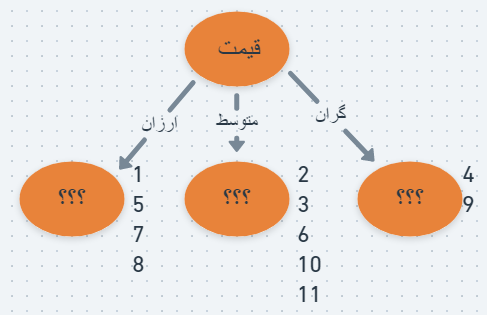
\includegraphics[width=0.5\textwidth]{dt1.png}
	\end{figure}
	در مرحله‌ی بعد داده‌هایی که به سمت گران دسته‌بندی  می‌شوند همه یک برچسب خورده‌اند بنابراین این راس به برگ تبدیل شده و مقدار برچسب $0$ می‌گیرد. برای راس ارزان، داده‌ها \lr{IG} برابری دارند بنابراین یکی از آن‌ها را به صورت تصادفی انتخاب کرده‌ایم که ویژگی \textbf{نوع غذا} بوده است. برای راس متوسط نیز \lr{IG} ویژگی \textbf{مکان} بیش‌تر بوده و این ویژگی انتخاب شده است. درخت بعد از این مرحله به شکل زیر در می‌آید:
	\begin{figure}[H]
		\centering
		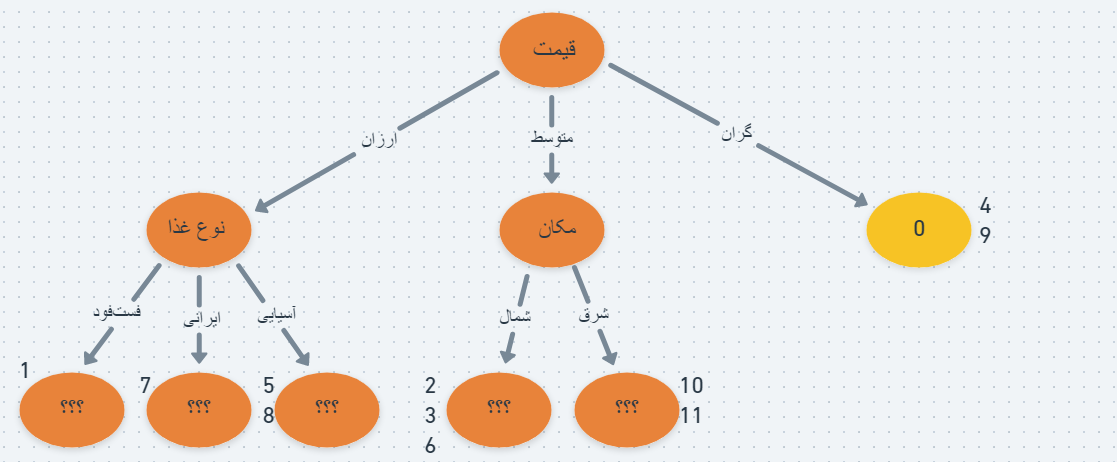
\includegraphics[width=0.9\textwidth]{dt2.png}
	\end{figure}
	در این مرحله راس‌هایی که یک داده برای آن‌ها مانده برچست همان داده را می‌گیرند. داده‌های 10 و 11 نیز برچسب یکسانی دارند بنابراین راس آن‌ها نیز همان برچسب آن‌ها یعنی $1$ را خواهد گرفت. برای مابقی راس‌ها از میان ویژگی‌های باقی مانده، آن ویژگی که \lr{IG} بیش‌تری داشته باشد را انتخاب می‌کنیم. برای داده‌های 5 و 8، ویژگی‌های باقی‌مانده «مکان» و «محدودیت» هستند که هر دو نیز \lr{IG} یکسانی دارند بنابراین به صورت تصادفی \textbf{مکان} انتخاب شده است. برای داده‌های 2،3 و 6، \textbf{نوع غذا} بیش‌ترین \lr{IG} را دارد. پس از این تقسیم‌بندی راس‌های باقی مانده یک داده خواهند داشت و در نتیجه به برگ تبدیل می‌شوند. درخت تصمیم در نهایت به صورت زیر در خواهد آمد:
	\begin{figure}[H]
		\centering
		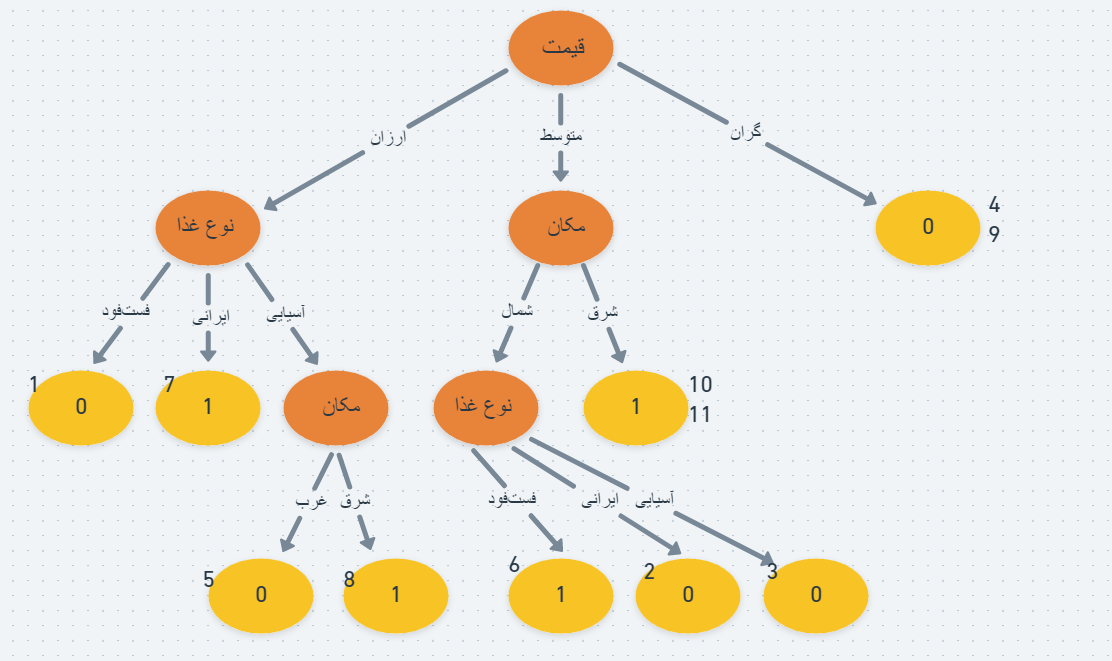
\includegraphics[width=0.95\textwidth]{dt3.png}
	\end{figure}
	\item
	با استفاده از درختی که در قسمت (آ) بدست آوردیم داریم:
	\[
	\begin{dcases}
		\text{رضایت‌مندی}(12) = 0 \\
		\text{رضایت‌مندی}(13) = 1 \\
		\text{رضایت‌مندی}(14) = 1 \\
		\text{رضایت‌مندی}(15) = 1 \\
		\text{رضایت‌مندی}(16) = 1
	\end{dcases}
	\]
	\item
	برای بدست آوردن
	$F_1 \text{Score}$
	نیاز به $recall$ و $precision$ داریم. برای این پارامترها نیز خواهیم داشت:
	\[
	\begin{dcases}
		recall = \frac{TP}{TP + FN} = \frac{2}{2 + 0} = 1\\[0.4em]
		precision = \frac{TP}{TP + FP} = \frac{2}{2 + 2} = 0.5
	\end{dcases}
	\]
	بنابراین برای 
	$F_1 \text{Score}$
	داریم:
	\[
	F_1 \text{Score} = \frac{2\times precision \times recall}{precision + recall} = \frac{2 \times 0.5 \times 1}{0.5 + 1} = \frac{2}{3}
	\]
\end{enumerate}
\pagebreak
\section*{سوال ۵}
\begin{enumerate}[A)]
	\item
	با توجه به استقلال داده‌ها از یکدیگر، درست‌نمایی را می‌توان به صورت زیر نوشت:
	\[
	\prob\{\mathcal{D}\,|\,\pi_1, \cdots, \pi_K\} = \prod_{i=1}^{N} \prob\{\mathcal{D}_i \,|\, \pi_1, \cdots, \pi_K\}  \quad(\ast)
	\]
	که با توحه به این‌که
	$\mathcal{D} = \{\phi_n, t_n\}_{i=1}^{N}$
	، برای احتمال دیدن یک داده خواهیم داشت:
	\[
	\prob\{t_i \,|\, \pi_1, \cdots, \pi_K\} = \pi_j, \quad (t_i)_j = 1 \quad(\star)
	\]
	بنابراین احتمال دیدن هر داده برابر با خواهد بود با $\pi_k$ که $k$ کلاسی‌ست که به آن تعلق دارد. حال اگر $N_i$ تعداد داده‌هایی باشد که به کلاس $i$ام تعلق دارند، با توجه به $(\ast)$ و $(\star)$ برای احتمال دیدن $\mathcal{D}$ خواهیم داشت:
	\[
	\prob\{\mathcal{D}\,|\,\pi_1,\cdots,\pi_K\} = \prod_{i=1}^K \pi_i^{N_i}
	\]
	برای پیدا کردن تخمین‌گر $\pi_i$ از لگاریتم تابع درست‌نمایی استفاده می‌کنیم. بنابراین داریم:
	\[
	\ln\left(\prob\{\mathcal{D}\,|\,\pi_1,\cdots,\pi_K\}\right) = \sum_{i=1}^K N_j\ln(\pi_j)
%	\begin{aligned}
%		\ln\left(\prob\{\mathcal{D}\,|\,\pi_1,\cdots,\pi_K\}\right) &= \sum_{i=1}^{N}\ln\left(\prod_{j=1}^{K} \pi_j^{(t_i)_j}\right) \\[0.7em]
%			&= \sum_{i=1}^{N} \left(\sum_{j=1}^{K} (t_i)_j\ln(\pi_j)\right) \\[0.7em]
%			&= \sum_{j=1}^K \left(\sum_{i=1}^N (t_i)j\ln(\pi_j)\right) \\[0.7em]
%			&= \sum_{j=1}^K N_j\ln(\pi_j)
%	\end{aligned}
	\]
	که $N_j$ تعداد داده‌هایی‌ست که در کلاس $j$ام دسته‌بندی شده‌اند. برای پیداکردن $\pi_i$هایی که عبارت بالا را بیشینه می‌کنند، شرط دیگری نیز داریم و آن هم یک شدن جمع همه‌ی آن‌ها یا به عبارتی
	$\sum_{j=1}^{K}\pi_j = 1$
	است. برای پیدا کردن بیشینه از روش ضرایب لاگرانژ استفاده می‌کنیم. تابع لاگرانژ به صورت زیر خواهد بود:
	\[
	L(\pi_1,\cdots,\pi_K, \lambda) = \sum_{j=1}^{K}N_j\ln(\pi_j) - \lambda \big(\sum_{j=1}^K \pi_j - 1\big)
	\]
	بنابراین برای مشتقات داریم:
	\[
	\begin{dcases}
		\frac{\partial L}{\partial \pi_j} = \frac{N_j}{\pi_j} - \lambda \\
		\frac{\partial L}{\partial \lambda} = -\sum_{j=1}^K \pi_j + 1
	\end{dcases}
	\]
	معادلات بالا را برابر صفر قرار داده و با بازنویسی رابطه‌ی اول خواهیم داشت:
	\[
	\begin{aligned}
		N_j = \lambda\pi^\ast_j &\xRightarrow{\sum_{j=0}^K} \lambda = N \\
		&\implies \boxed{\pi^\ast_j = \frac{N_j}{N}}
	\end{aligned}
	\]
	\item
	فرض کنیم $\mathcal{C}_i$ مجموعه‌ی شامل اندیس داده‌هایی باشد که کلاس مربوط به آن‌ها $i$ است. هم‌چنین $\bm{\mu}$ بردار شامل $\mu_k$ها بوده و $\bm{\pi}$ بردار شامل $\pi_k$ها باشد. با توجه به استقلال داده‌ها برای درست‌نمایی خواهیم داشت:
	\[
	\prob\{\mathcal{D}\,|\,\bm{\mu}, \Sigma, \bm{\pi}, \Phi\} = \prod_{i=1}^N\prob\{t_i \,|\, \bm{\mu}, \Sigma, \bm{\pi}, \phi_i\}
	\]
	که با توجه به تعریف $\mathcal{C}_i$ها خواهیم داشت:
	\[
	\prob\{\mathcal{D}\,|\,\bm{\mu}, \Sigma, \bm{\pi}, \Phi\} = \prod_{j=1}^K\left(\prod_{i\in \mathcal{C}_j} \prob\{\mathcal{C}_j \,|\, \bm{\mu}, \Sigma, \bm{\pi}, \phi_i\}\right)
	\]
	که احتمال داخل پرانتز بالا را نیز می‌توان به صورت زیر نوشت که $d$ بعد ویژگی‌هاست:
	\[
	\begin{aligned}
		\prob\{\mathcal{C}_j \,|\, \bm{\mu}, \Sigma, \bm{\pi}, \phi_i\} &= \prob(\mathrm{C}_j)\prob\{\phi_i\,|\, \mathcal{C}_j, \bm{\mu}, \Sigma\} \\
		&= \pi_j (2\pi)^{-\frac{d}{2}}|\Sigma|^{-\frac{1}{2}} \exp\left(-\frac{1}{2}(\phi_i-\mu_j)^T\Sigma^{-1}(\phi_i-\mu_j)\right)
	\end{aligned}
	\]
	از بیشینه کردن لگاریتم درست‌نمایی استفاده می‌کنیم:
	\[
	\begin{aligned}
	f(\bm{\mu}, \Sigma) &= \ln\left(\prob\{\mathcal{D}\,|\,\bm{\mu}, \Sigma, \bm{\pi}, \Phi\}\right) \\
	&= \sum_{j=1}^k N_j\ln(\pi_j) - \frac{Nd}{2}\ln(2\pi) - \frac{N}{2}\ln(|\Sigma|) - \frac{1}{2} \sum_{j=1}^K \left(\sum_{i\in \mathcal{C}_j}(\phi_i-\mu_j)^T\Sigma^{-1}(\phi_i-\mu_j)\right)
	\end{aligned}
	\]
	برای مشتق تابع بالا نسبت به $\bm{\mu}$ و $\Sigma$ خواهیم داشت:
	\[
	\begin{dcases}
		\frac{\partial f}{\mu_j} = -\frac{1}{2}\sum_{i\in \mathcal{C}_j} 2\Sigma^{-1}(\phi_i-\mu_j) \\
		\frac{\partial f}{\partial \Sigma} = -\frac{N}{2}\Sigma^{-1} + \frac{1}{2} \sum_{j=1}^K \left(\sum_{i\in \mathcal{C}_j}(\phi_i-\mu_j)(\phi_i-\mu_j)^T\Sigma^{-1}\Sigma^{-1}\right)
	\end{dcases}
	\]
	با صفر قرار دادن معادلات بالا برای $\mu^\ast_j$ و $\Sigma^\ast$ خواهیم داشت:
	\[
	N_j\mu_j^\ast = \sum_{i\in \mathcal{C}_j}\phi_i \implies \boxed{\mu^\ast_j = \frac{\sum_{i\in \mathcal{C}_j}\phi_i}{N_j}}
	\]
	\[
	\boxed{\Sigma^\ast = \dfrac{\sum_{j=1}^K\left(\sum_{i\in \mathcal{C}_j}(\phi_i-\mu_j)(\phi_i-\mu_j)^T\right)}{N}}
	\]
\end{enumerate}

\end{document}



